% Copyright 2004 by Till Tantau <tantau@users.sourceforge.net>.
%
% In principle, this file can be redistributed and/or modified under
% the terms of the GNU Public License, version 2.
%
% However, this file is supposed to be a template to be modified
% for your own needs. For this reason, if you use this file as a
% template and not specifically distribute it as part of a another
% package/program, I grant the extra permission to freely copy and
% modify this file as you see fit and even to delete this copyright
% notice. 

\documentclass{beamer}
\mode<presentation> {
% There are many different themes available for Beamer. A comprehensive
% list with examples is given here:
% http://deic.uab.es/~iblanes/beamer_gallery/index_by_theme.html
% You can uncomment the themes below if you would like to use a different
% one:
%\usetheme{AnnArbor}
%\usetheme{Antibes}
%\usetheme{Bergen}
%\usetheme{Berkeley}
%\usetheme{Berlin}
%\usetheme{Boadilla}
%\usetheme{boxes}
%\usetheme{CambridgeUS}
%\usetheme{Copenhagen}
%\usetheme{Darmstadt}
%\usetheme{default}
%\usetheme{Frankfurt}
%\usetheme{Goettingen}
%\usetheme{Hannover}
%\usetheme{Ilmenau}
%\usetheme{JuanLesPins}
%\usetheme{Luebeck}
\usetheme{Madrid}
%\usetheme{Malmoe}
%\usetheme{Marburg}
%\usetheme{Montpellier}
%\usetheme{PaloAlto}
%\usetheme{Pittsburgh}
%\usetheme{Rochester}
%\usetheme{Singapore}
%\usetheme{Szeged}
%\usetheme{Warsaw}
}

\usepackage{graphicx} 
\usepackage{booktabs} 
\usepackage[portuguese]{babel}
\usepackage[utf8]{inputenc}
\usepackage{multicol}
\usepackage{blindtext}

\title{Análise Estatística Aplicada à Teoria Coalescente e Modelagem Ecológica}

% A subtitle is optional and this may be deleted
%\subtitle{Teoria }

\author{Willian M. S.\inst{1} \and Sandro P. F.\inst{2}}
% - Give the names in the same order as the appear in the paper.
% - Use the \inst{?} command only if the authors have different
%   affiliation.

\institute[UFPR] % (optional, but mostly needed)
{
  \inst{1}%
  Aluno de Graduação - Bolsista Pet\\
  Departmento de Estatística - UFPR
  \and
  \inst{2}%
  Aluno PhD - PPG Zoology\\
  Laboratory of Ecology and Evolution of Interactions - UFPR
  }
% - Use the \inst command only if there are several affiliations.
% - Keep it simple, no one is interested in your street address.

\date{\today}

%\subject{Theoretical Computer Science}

\AtBeginSubsection[]
{
  \begin{frame}<beamer>{Indice}
    \tableofcontents[currentsection,currentsubsection]
  \end{frame}
}

% Let's get started
\begin{document}

%---------------------------
\begin{frame}
\titlepage % Print the title page as the first slide
\end{frame}
%---------------------------



%---------------------------
\begin{frame}
\frametitle{Pesquisa Individual} % Table of contents slide, comment this block out to remove it
\tableofcontents % Throughout your presentation, if you choose to use \section{} and \subsection{} commands, these will automatically be printed on this slide as an overview of your presentation
\end{frame}

%----------------------------------------------------------------------------------------
%	PRESENTATION SLIDES
%----------------------------------------------------------------------------------------

%------------------------------------------------
\section{Teoria Coalescente} % Sections can be created in order to organize your presentation into discrete blocks, all sections and subsections are automatically printed in the table of contents as an overview of the talk
%------------------------------------------------

% OK *********************************************************************************
\subsection{Introdução}
    \begin{frame}{Introdução}

        \begin{block}{Motivação}
            Através de modelos de relação ancestral-descendentes (genealogias) é possível identificar através de amostras de DNA, padrões nos indivíduos do presente e inferir a identidade no passado por descendência e reconstruir eventos históricos
        \end{block}
          
    
    \end{frame}
% OK *********************************************************************************
% OK *********************************************************************************
\subsection{Metodologia}
    \begin{frame}{Metodologia}
        %\textbf{Objetivos}
        \begin{itemize}
            \item Coletado uma amostra de uma espécie, onde não sabemos nada sobre suas genealógia
            \item O DNA é codificado e sequenciado
                \begin{itemize}
                    \item Quatro bases proteícas (A, T, C, G)
                \end{itemize}   
            \item Análise dos polimorfismos das amostras de populações naturais
            \item Aprender algo sobre os eventos passados da genética das populações
            \begin{itemize}
                \item Modelos de relação ancestral-descendentes (genealogias)
            \end{itemize} 
            \item Interpretar as seqüências e dar-lhes um sentido evolutivo
        \end{itemize} 
 
     \end{frame}
% OK *********************************************************************************
% OK *********************************************************************************
\subsection{Exemplos}
    \begin{frame}{Cadeia DNA}
        \begin{figure}[!h]
            \centering
            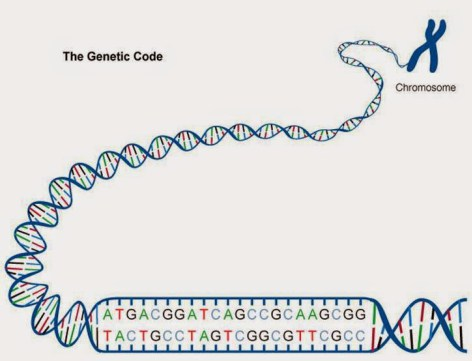
\includegraphics[scale=0.35]{dnacod.jpg} \quad
            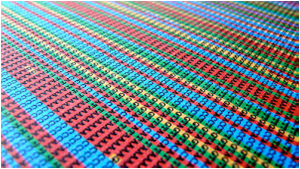
\includegraphics[scale=0.35]{Imagem2.png}
            \caption{Cadeia genética sequenciada}
            \label{Rotulo}
        \end{figure}
   \end{frame}

   \begin{frame}{Coalescencia}
        \begin{figure}[!h]
            \centering
            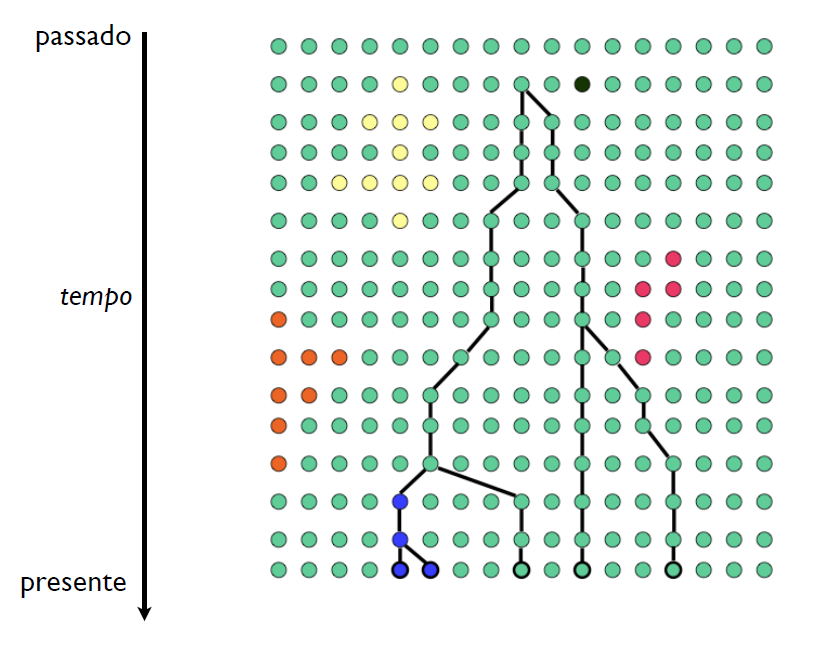
\includegraphics[scale=0.3]{coal.png}
            \caption{Representação de uma árvore de evolução}
            \label{Rotulo}
        \end{figure}
   \end{frame}

\begin{frame}{Relação Mutação x Tempo}
    \begin{figure}[!h]
        \centering
        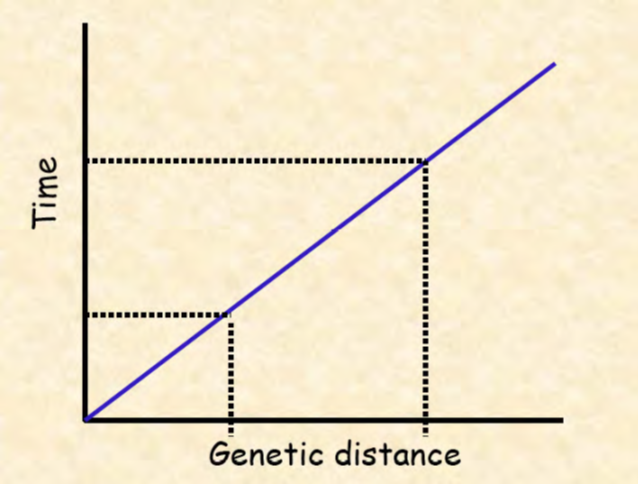
\includegraphics[scale=0.4]{timegen.png} \quad
	      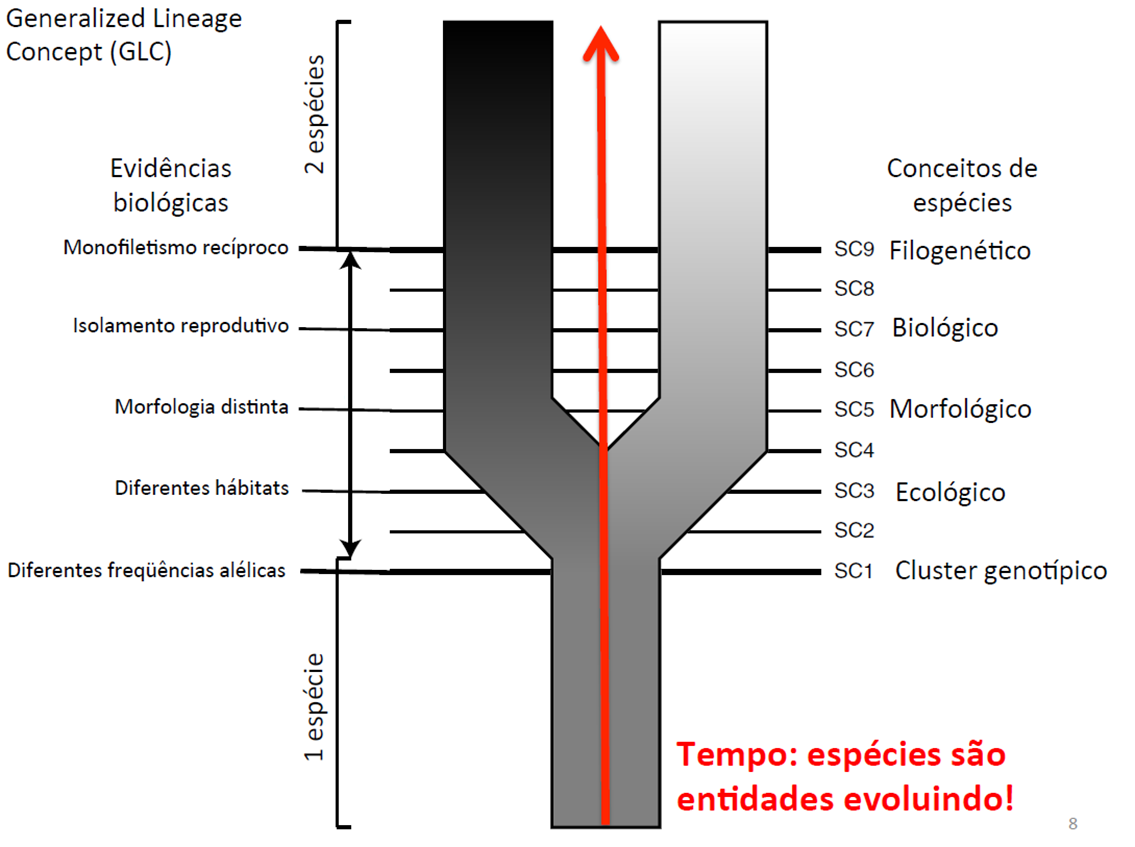
\includegraphics[scale=0.3]{timegen2.png}
        \caption{Relação Mutação x Tempo}
        \label{Rotulo}
    \end{figure}
\end{frame}

\section{Habitat Estudado}
%------------------------------------------------
  \subsection{Região}
    \begin{frame}{Região}
        %\textbf{Espécies}
      \begin{figure}[!h]
          \centering
          %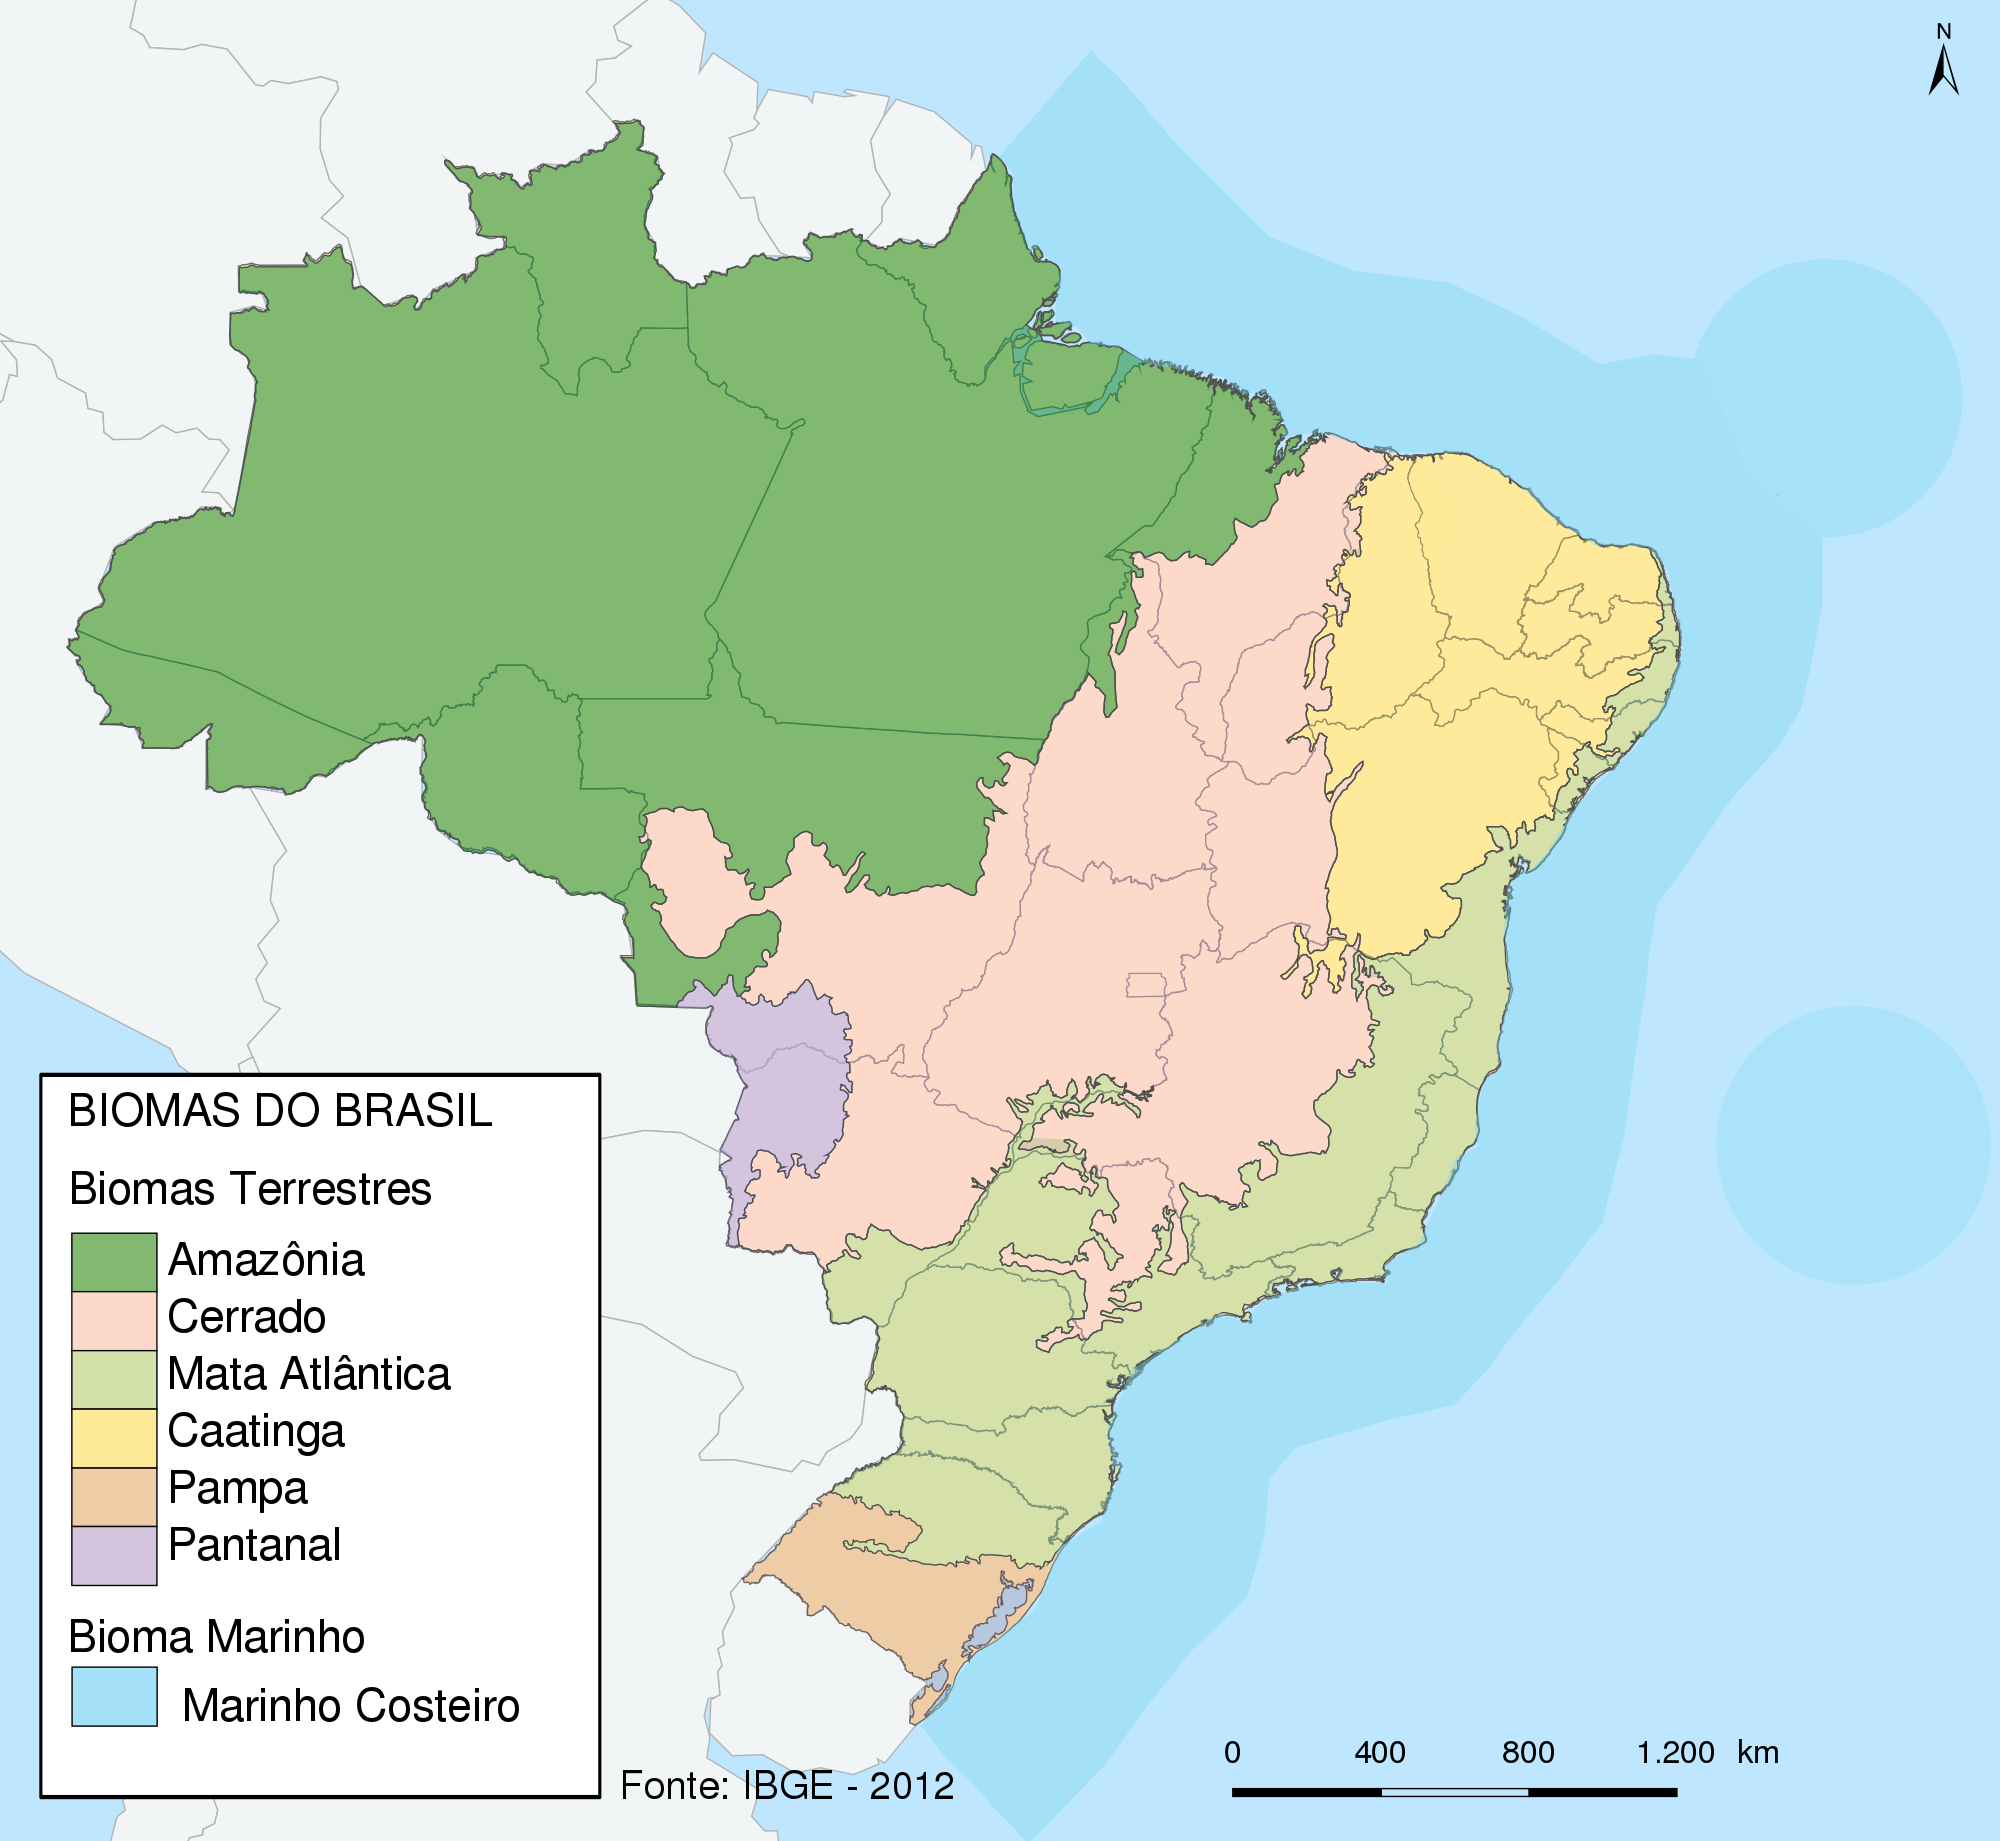
\includegraphics[scale=0.07]{regiao2.png}\quad
  	      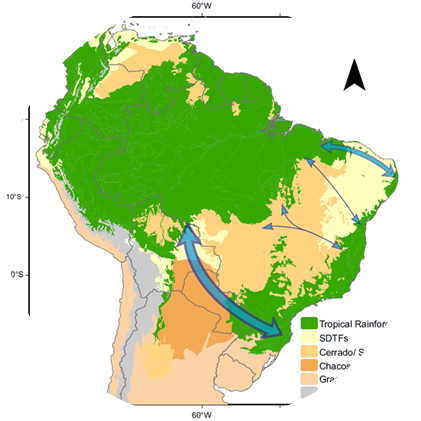
\includegraphics[scale=0.7]{diagseca2.png}\quad
  	      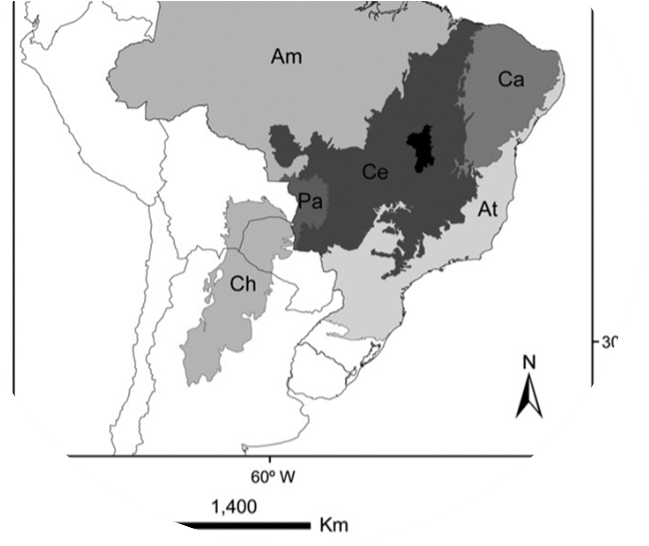
\includegraphics[scale=0.5]{diagseca.png}
          \caption{Diagonal seca da América do Sul}
          \label{Rotulo}
      \end{figure}
    \end{frame}
    
    \begin{frame}{Região}
        %\textbf{Espécies}
      \begin{figure}[!h]
          \centering
          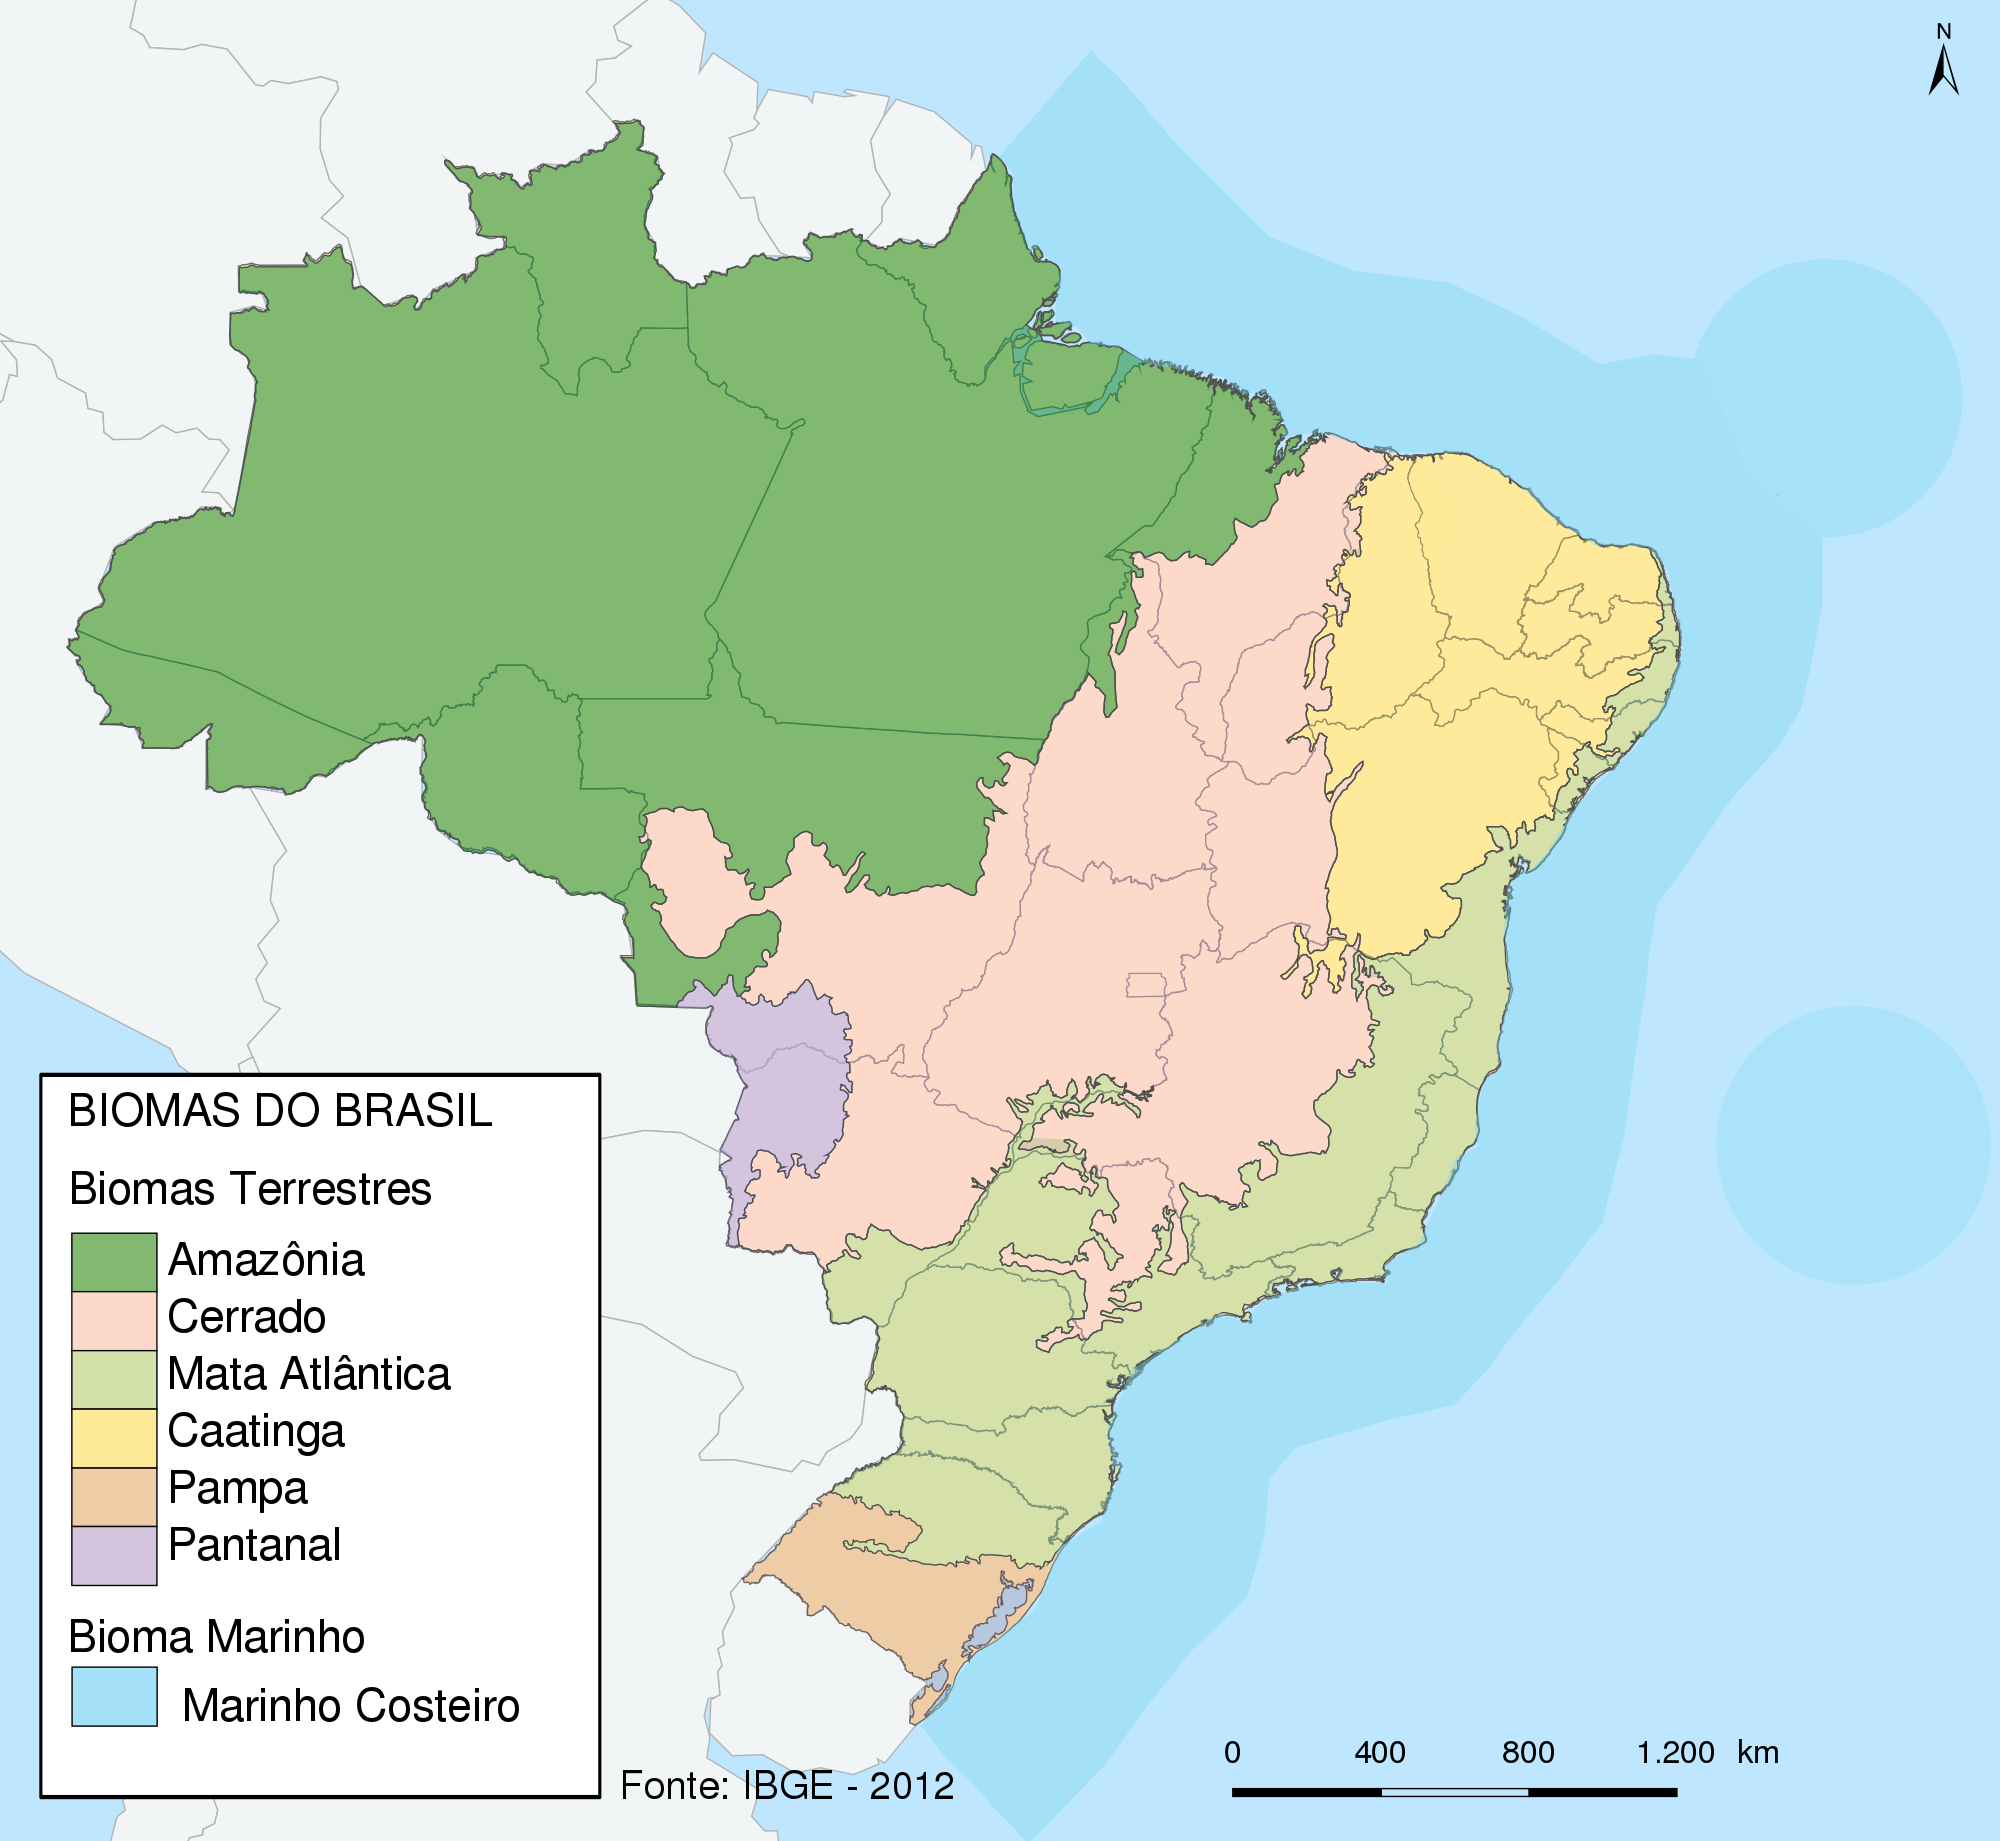
\includegraphics[scale=0.1]{regiao2.png}
  	      \caption{Diagonal seca da América do Sul}
          \label{Rotulo}
      \end{figure}
    \end{frame}    
 
  \subsection{Espécies}
    \begin{frame}{Espécies}
        %\textbf{Espécies}
        \begin{itemize}
            \item Beija-Flor (Anopetia gounellei)
            \item Pica-Pau (Picullus chrysochloros)
            \item Rã-Manteiga (Leptodactylus latrans )
        \end{itemize}
        \begin{figure}[!h]
          \centering
          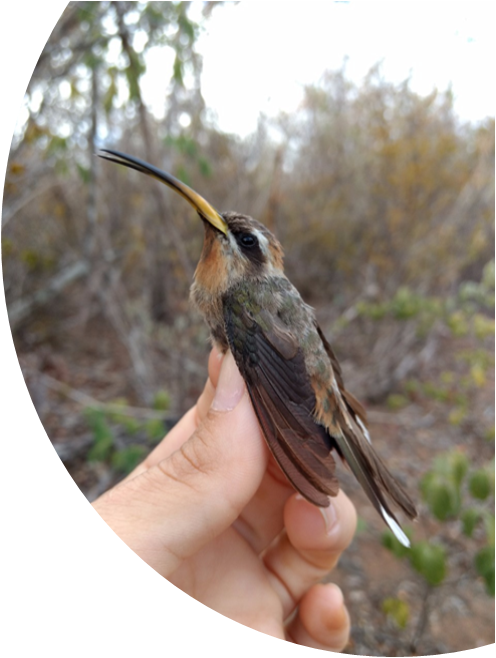
\includegraphics[scale=0.28]{bf1.png} \quad
  	      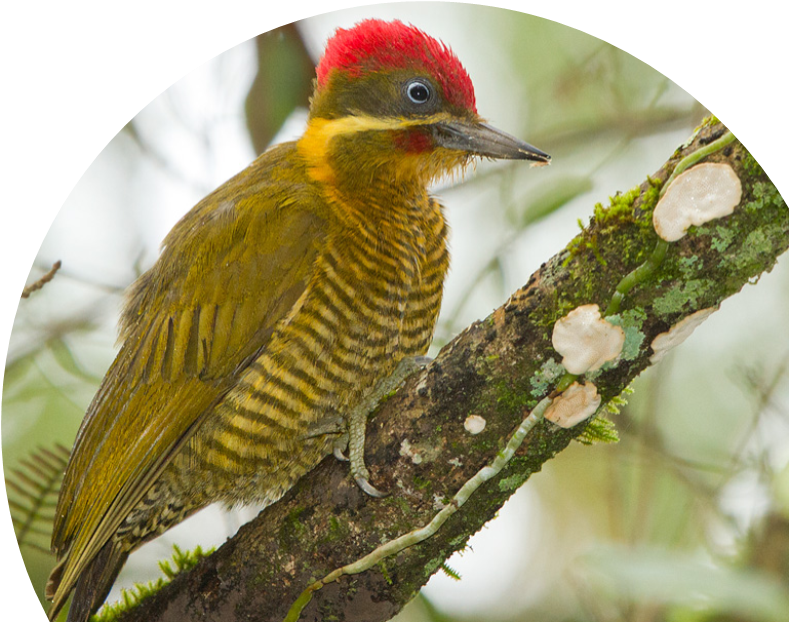
\includegraphics[scale=0.25]{PP1.png}\quad
  	      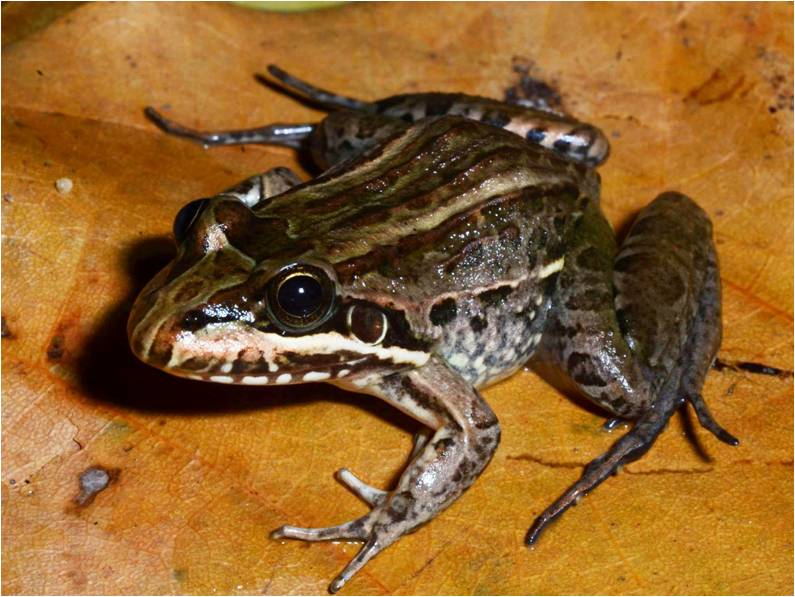
\includegraphics[scale=0.3]{ra.jpg}
          %\caption{Relação Mutação x Tempo}
          \label{Rotulo}
        \end{figure}
    \end{frame}
    
% OK *********************************************************************************
\subsection{Beija-Flor}
    \begin{frame}{Beija-Flor - Evolução}
        \begin{figure}[!h]
          \centering
          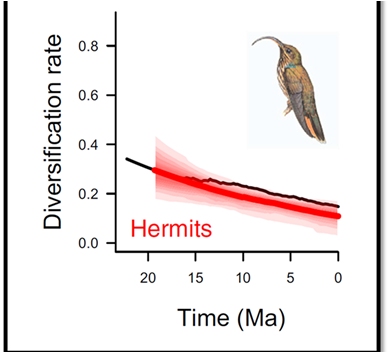
\includegraphics[scale=0.28]{bf-timepng.png} \quad
  	      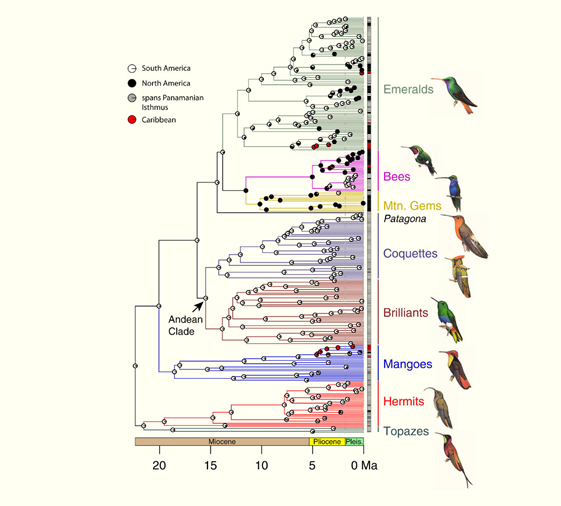
\includegraphics[scale=0.75]{bf_geneal.png}
          %\caption{Relação Mutação x Tempo}
          \label{Rotulo}
        \end{figure}    
    \end{frame}
    
    \begin{frame}{Beija-Flor - Região}
        \begin{figure}[!h]
          \centering
  	      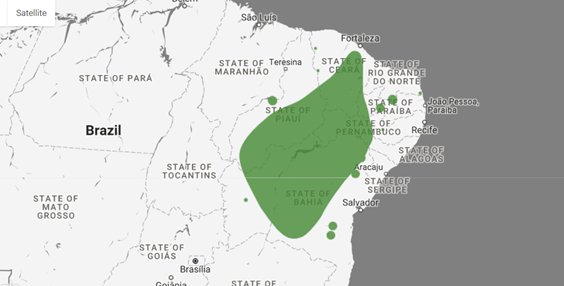
\includegraphics[scale=1.0]{bf_regiao.png}
          \caption{Habitat desta espécie de beija-flor}
          \label{Rotulo}
        \end{figure}    
    \end{frame}

\begin{frame}
    \Huge{\centerline{Obrigado pela atenção!!}}
\end{frame}

\end{document}


